% Distributed Cyber-Resilience for Containerized Healthcare Applications
% IEEE journal-format source. Build: pdflatex main && pdflatex main (no BibTeX needed, references are inline).
% Not compiled in the environment where it was written; see README.md in this folder.
\documentclass[journal]{IEEEtran}

\usepackage{cite}
\usepackage{amsmath}
\usepackage{graphicx}
\usepackage{booktabs}
\usepackage{array}
\usepackage{tabularx}
\usepackage{url}
\usepackage{textcomp}
\usepackage{fancyhdr}
\newcommand{\runhead}{\footnotesize B.M.S.\ College of Engineering, Department of Computer Science Engineering, November 2026}
\setlength{\headheight}{14pt}
\pagestyle{fancy}
\fancyhf{}
\lhead{\runhead}
\rhead{\footnotesize\thepage}
\renewcommand{\headrulewidth}{0pt}
\fancypagestyle{plain}{\fancyhf{}\lhead{\runhead}\rhead{\footnotesize\thepage}\renewcommand{\headrulewidth}{0pt}}

\graphicspath{{figs/}}
\newcommand{\stage}[1]{\texttt{#1}}
\newcommand{\action}[1]{\texttt{#1}}
\newcolumntype{Y}{>{\raggedright\arraybackslash}X}

\begin{document}

\title{Distributed Cyber-Resilience for Containerized Healthcare Applications}

\author{%
\small
\setlength{\tabcolsep}{2pt}
\begin{tabular}{*{5}{>{\centering\arraybackslash}p{3.3cm}}}
Swetha P.\,C. & Idrees Shaikh & Karan Nair & Manish Ramu & Mohammed Amaan\\
\textit{Associate Professor} & \textit{B.E.\ Student} & \textit{B.E.\ Student} & \textit{B.E.\ Student} & \textit{B.E.\ Student}\\
\textit{Information Science Engineering} & \textit{Computer Science Engineering} & \textit{Computer Science Engineering} & \textit{Computer Science Engineering} & \textit{Computer Science Engineering}
\end{tabular}}

\maketitle
\thispagestyle{fancy}

\begin{abstract}
Containerized healthcare applications running on Kubernetes consist of numerous small components, and a breach of any single component, or of its monitor, can disrupt the entire application. Most intrusion detection and response solutions still rely on a single point of decision-making or on individual alerts, so a false or corrupted alert can lead to disruptive action. In this paper, we introduce a prototype in which four peer security agents monitor six logical workloads of a healthcare application using network, process, file-integrity and authentication indicators. The agents exchange Ed25519-signed evidence over gRPC with mutual TLS, maintain their own trust score for each peer, and weigh the evidence by that score. A protective action requires signed votes from at least three distinct eligible agents. This is an application-level threshold scheme, not a Byzantine fault-tolerant consensus protocol. An approved containment creates a forensic snapshot, isolates the workload with a Kubernetes NetworkPolicy, restores it from a known-good image, validates that the replacement is healthy, and puts the workload back into service through a five-stage process. Of 80 simulated runs, the workload regained full access in all 80, with a median time to isolate of 1.2~s. A single lying agent never isolated a healthy workload (0/20), while three compromised agents did (20/20). Furthermore, with only two agents alive, nothing could be isolated at all. The detector is simplistic: in a mixed run, 29 of 30 benign transients triggered an alarm and 15 of them led to an isolation. A four-node Minikube/Calico sandbox completed one contain--replace--validate--reintegrate cycle in 83~s.
\end{abstract}

\begin{IEEEkeywords}
Collaborative intrusion detection, container security, cyber-resilience, trust management, quorum authorization, Kubernetes, healthcare.
\end{IEEEkeywords}

\section{Introduction}
\IEEEPARstart{H}{ospitals} and health technology providers operate patient portals, record services, laboratory information systems and databases managed by Kubernetes. This simplifies scaling and upgrades; it also makes the application an architecture of small services that may be exploited, messed up, or brought down. An outage or a breach in this environment has two consequences: availability and privacy issues.

An intrusion detector operating from one perspective has two problems known to everybody. The first is that the detector and controller are vulnerable to attack, which would render the entire system useless. The second is that a response driven by a single alert will eventually be triggered by a false alert. Distributed detection, where monitors share information, helps with the first problem~\cite{zhou10,vasilo15,li22}; it introduces another issue. A monitor may be authenticated but could still be wrong or malicious.

Our prototype considers these two issues separately. Messages are authenticated through signatures and mutual TLS, while the trust in each sender is evaluated independently as a trust score that every agent maintains for itself. A disruptive action is only performed when three out of the four agents agree. After containment, the workload is restored from the known-good image and brought back incrementally in stages, rather than all at once.

Our contributions are limited, but relate to integration:
\begin{enumerate}
\item A distributed architecture consisting of four identical peer agents monitoring six containerized healthcare workloads with no central controller.
\item An evidence path incorporating Ed25519 signatures, gRPC over mutual TLS, trust scores per observer, and a trust-weighted score for deciding how to vote.
\item A three-of-four threshold-based authorization for containment, validation, recovery attempts and each reintegration step, validated through signed quorum certificates and a Kubernetes admission webhook.
\item An evaluation split into a simulator that runs the actual agent code and a four-node Minikube/Calico sandbox. We state where the design succeeds and where it fails: three compromised agents, two agents alive, and a noisy detector.
\end{enumerate}
We do not claim that any one of the mechanisms discussed in this paper is novel. The quorum is not a Byzantine fault-tolerant protocol, the detector relies on rule-based detection without any kind of learning, and the data are artificial. The limitations are listed in Section~\ref{sec:limits}.

Section~II contains an overview of related work. Section~III covers the system description. Section~IV describes the experiments. Section~V presents the results, Section~VI covers the limitations, and Section~VII concludes.

\section{Related Work}
\subsection{Collaborative intrusion detection}
Zhou et al.~\cite{zhou10} surveyed coordinated attacks and collaborative detection and observed that sharing observations between monitoring points reveals attacks that cannot be seen by a single host. Vasilomanolakis et al.~\cite{vasilo15} studied collaborative systems according to their architecture and coordination and raised issues of information sharing and trust. Li et al.~\cite{li22} reviewed trust-based collaborative detection. Regarding the correlation aspect, Elshoush and Osman~\cite{elshoush11} presented a survey on alert correlation, while Balasubramaniyan et al.~\cite{balas98} proposed a cooperative detection architecture using autonomous agents. These works provide motivation for sharing information between monitoring agents, but mostly stop there, and do not consider the workload following the alert.

\subsection{Trust and reputation}
J{\o}sang et al.~\cite{josang07} reviewed trust and reputation systems, while Kamvar et al.~\cite{kamvar03} proposed the EigenTrust model, where global reputations are calculated from peer feedback. We have taken a different approach. Each agent calculates its own trust towards its peers, and changes it only when the peer reports something different from what the agent sees. There is no global reputation to be attacked.

\subsection{Byzantine fault tolerance}
The Byzantine generals problem~\cite{lamport82} and the impossibility result for asynchronous consensus with one faulty process~\cite{flp85} define the scope of agreement between unreliable entities. PBFT~\cite{castro99,castro02} supports $f$ Byzantine replicas, with $n=3f+1$ replicas and quorums of $2f+1$; for $n=4$ and $f=1$ that quorum size is three. We use those parameters too, but only for configuration. Our mechanism has no leader, no views, no ordered log and no pre-prepare/prepare/commit steps, hence it does not offer any of PBFT's guarantees.

\subsection{Container and cloud security}
Jarkas et al.~\cite{jarkas25} summarize container attacks and defenses; Patel et al.~\cite{patel13} and Modi et al.~\cite{modi13} review cloud intrusion detection and prevention mechanisms; NIST SP~800-190~\cite{nist190} offers container hardening best practices. The above-mentioned sources describe attacks and preventive measures. Our concern is the remedial part: containment, replacement and re-entry of the compromised workload.

\subsection{Anomaly detection, cryptography and incident response}
Anomaly-based detection is general and extensively surveyed~\cite{garcia09,bhuyan14,khraisat19}, but its major practical difficulty is false alarms. Our anomaly detector is intentionally simple: no modeling, only threshold values and rules, whose behaviour can be easily analyzed, and, as shown in Section~V, quite noisy. For message cryptography we use Ed25519 (EdDSA, RFC~8032~\cite{rfc8032}), TLS~1.3~\cite{rfc8446} and the X.509 profile~\cite{rfc5280}. For the response process we use the principles of NIST incident response guidelines~\cite{nist61}, zero trust architecture~\cite{nist207} and NIST Cybersecurity Framework~2.0~\cite{csf2}, although we do not claim compliance with any of them.

\subsection{Gap}
Every field listed above is extensively researched separately. We found fewer papers in which collaborative evidence, agent-level trust, threshold-based authorization and progressive recovery of a Kubernetes workload are combined in one prototype and tested against lying, crashed and colluding agents. Table~\ref{tab:related} below shows how our prototype relates to the research literature. The right column describes our approach rather than innovations.

\begin{table}[!t]
\caption{Related Work and What This Prototype Does}
\label{tab:related}
\centering\small
\begin{tabularx}{\columnwidth}{@{}p{1.9cm} Y Y@{}}
\toprule
Area & Literature & This prototype \\
\midrule
Collaborative IDS & Shared alerts and correlation~\cite{zhou10,vasilo15,elshoush11} & Four peers exchange signed evidence \\
Trust & Global reputation~\cite{josang07,kamvar03} & Per-observer trust, contradiction-driven \\
Agreement & PBFT~\cite{castro99,castro02} & Three-of-four threshold voting, no PBFT phases \\
Container security & Surveys and guidance~\cite{jarkas25,nist190} & NetworkPolicy isolation and image replacement \\
Detection & Anomaly surveys~\cite{garcia09,bhuyan14} & Fixed thresholds and rules, no learning \\
Authentication & EdDSA, TLS, X.509~\cite{rfc8032,rfc8446,rfc5280} & Ed25519 signatures plus mutual TLS \\
Response & Incident-response guidance~\cite{nist61,nist207} & Snapshot, isolate, replace, validate, staged return \\
\bottomrule
\end{tabularx}
\end{table}

\section{Proposed System}
\subsection{System description}
The system consists of four peer security agents, labeled A to D, that monitor six logical workloads labeled A to F (Fig.~\ref{fig:arch}). The agents are equal, and there is no leader among them. Workloads A to D each have their own co-located agent, whereas workloads E and F, which are the laboratory-results and medication services, do not and are monitored by all four agents. We will call the four decision makers ``agents'' and the six protected services ``workloads'' henceforth.

Each agent polls workload telemetry, generates signed evidence from it, sends the evidence to its peers, and judges what it receives based on its trust scores. When three distinct eligible agents vote for a single action, the action is authorized, a quorum certificate is created, and one agent, selected according to a fixed ranking, executes the action. Fig.~\ref{fig:flow} illustrates the process.

\begin{figure*}[!t]
\centering
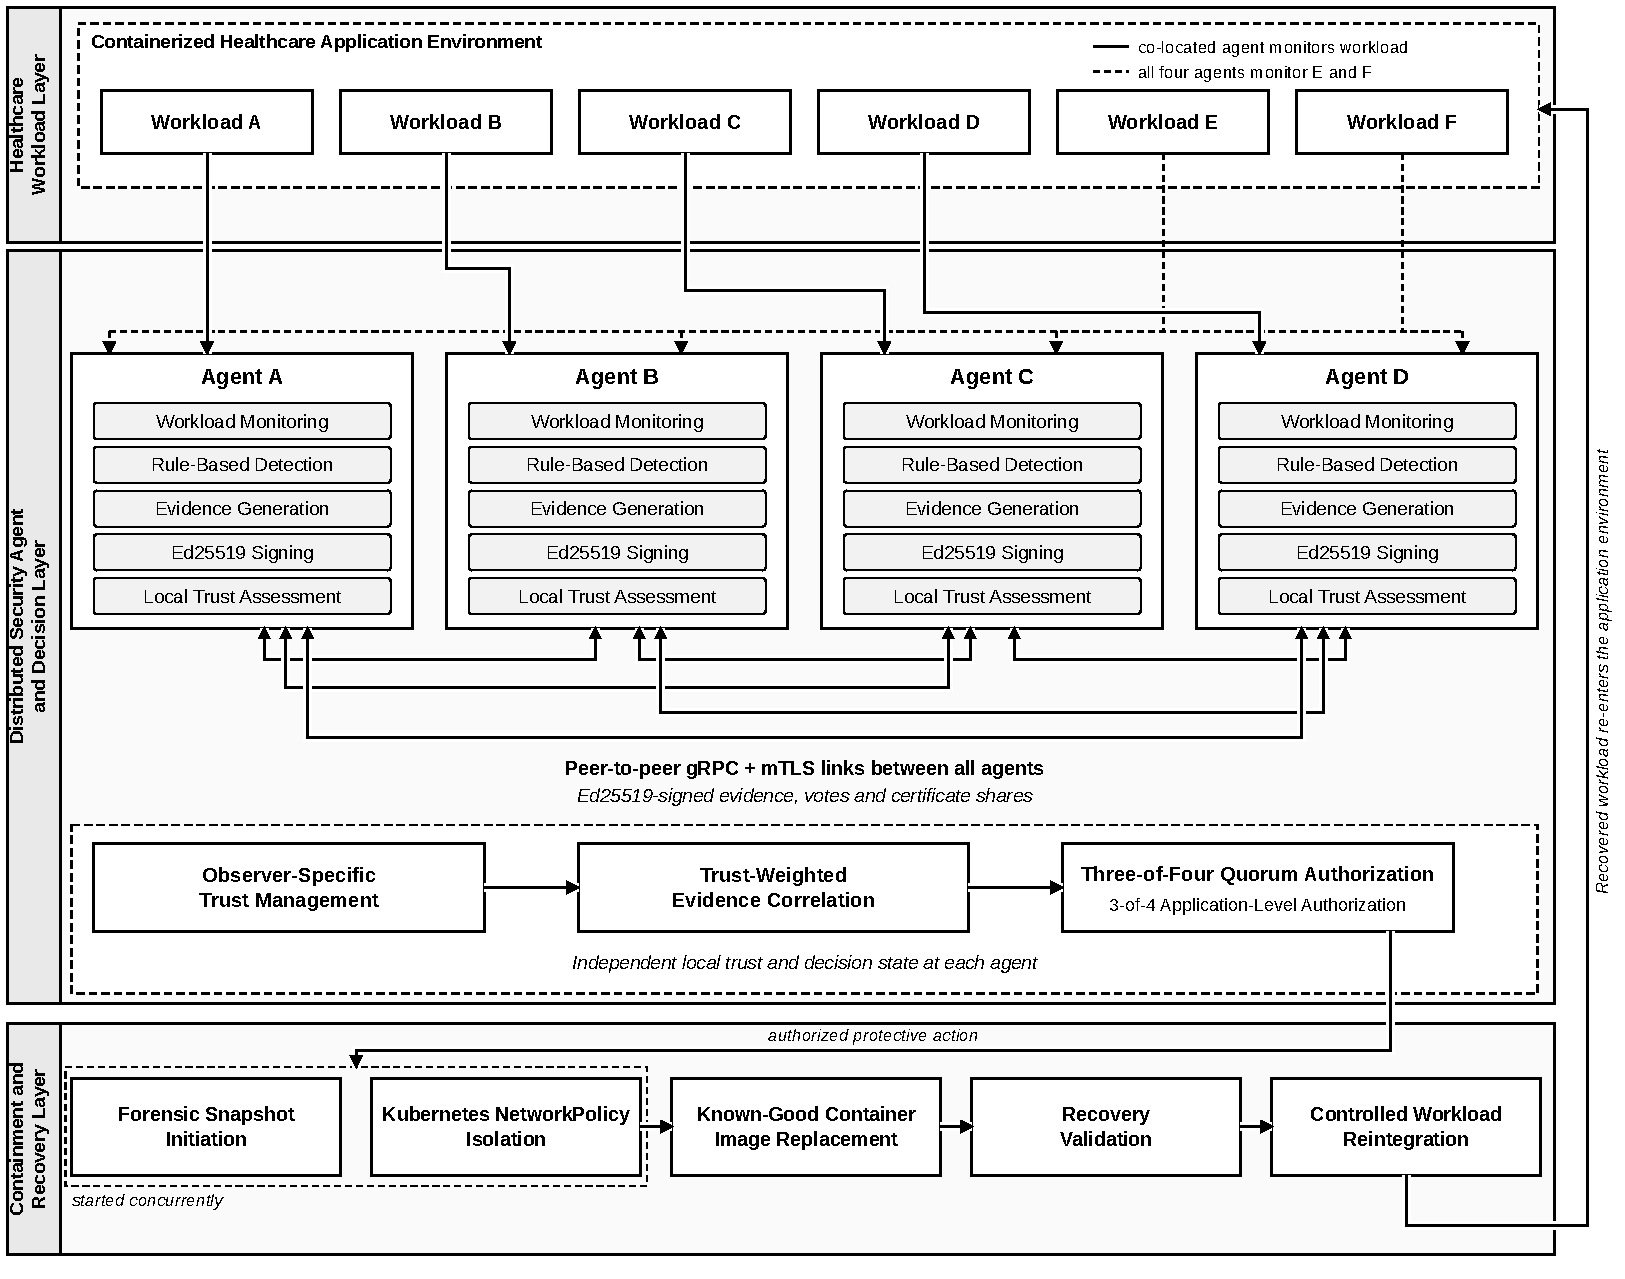
\includegraphics[width=0.92\textwidth]{fig1_architecture.pdf}
\caption{Overall architecture of the proposed distributed cyber-resilience system for containerized healthcare applications. Solid arrows show co-located monitoring; dashed arrows show that all four agents monitor workloads E and F.}
\label{fig:arch}
\end{figure*}

\subsection{Monitoring and evidence generation}
Rule-based detection works by checking four kinds of signal (Table~\ref{tab:signals}): network traffic sent by the workload (the number of outbound connections and the volume of data sent per second), the list of running processes, the integrity of files against a known-good SHA-256 manifest, and failed authentications from the workload's pod IP address. Anomalies are flagged by comparison with thresholds, and the amount by which a threshold is exceeded is expressed as a confidence. For the two network metrics and authentication failures, the confidence grows with the amount by which the metric exceeds its threshold:
\begin{equation}
c(x)=\begin{cases}
0, & x\le\theta,\\[2pt]
0.5+0.5\,\min\!\left(1,\dfrac{x-\theta}{s}\right), & x>\theta,
\end{cases}
\label{eq:conf}
\end{equation}
where $x$ is the measurement, $\theta$ the threshold, and $s$ a scale. The scales are 16 connections, $10^{6}$~B/s and 40 failed logins respectively. For process and file signals the confidence is fixed and defined by the matching rule. The thresholds have not been tuned or benchmarked; they are engineering defaults.

The evidence messages include the name of the agent, the target workload, the kind of signal, the confidence and the timestamp. It is important to note that workloads provide telemetry data themselves, including the file hashes, over HTTP inside the cluster. We depend on many agents analyzing the same workload, not on the information provided by any particular workload.

\begin{table}[!t]
\caption{Implemented Detection Conditions}
\label{tab:signals}
\centering\small
\begin{tabularx}{\columnwidth}{@{}l Y Y@{}}
\toprule
Signal & Condition & Parameter \\
\midrule
Network & Outbound connections & More than 8 \\
Network & Outbound transmit rate & More than 256\,000 B/s \\
Process & Suspicious name or directory & Confidence 0.95 \\
Process & Not in the allowlist & Confidence 0.60 \\
File integrity & Modified file & Confidence 0.95 \\
File integrity & Missing file & Confidence 0.80 \\
File integrity & New file & Confidence 0.70 \\
Authentication & Failed logins & More than 10 in 10\,s \\
\bottomrule
\end{tabularx}
\end{table}

\subsection{Evidence exchange}
Evidence, votes and certificate shares are Protocol Buffer messages enclosed in a signed envelope. The signature is Ed25519 over the message kind, a zero byte and the serialized payload; the kind prefix protects the signature from being reused for a different message type. Agents communicate over gRPC with mutual TLS; the certificate common name identifies the agent.

On receipt, an agent performs the following checks, in this order: that the TLS identity matches the claimed signer; that the signer is known; that the signature is valid; that the payload can be parsed and was authored by the signer; that the timestamp differs by less than 15\,s from the current local time; and that the message is not found in a 120\,s replay cache. Any message that fails a check is rejected and the peer that delivered it receives a penalty of 20 trust points. For evidence, the recipient then checks the trust value of the sender (next subsection).

Signature verification ensures that the message was indeed sent by the specific agent and was not tampered with. It does not ensure that what the agent says is correct, and thus trust is dealt with separately.

\subsection{Agent trust}
Each agent maintains a trust value from 0 to 100 for each of the other three agents, starting at 100. This value changes linearly:
\begin{equation}
T(t+\Delta t)=\min\{100,\;\max\{0,\;T(t)+r\,\Delta t\}\}.
\label{eq:trust}
\end{equation}
A peer's claim counts as contradicted when its confidence is 0.5 or higher, the claim is at least 8\,s old, and the receiving agent's own highest confidence for that workload around the time of the claim stayed below 0.2. While a peer's claims are contradicted, $r=-2.5$ per second; otherwise $r=+0.5$ per second. Rejection of a message gives a one-time penalty of 20 points. Recovery is thus intentionally slower than the loss of trust.

There are two thresholds, and their functions differ:
\begin{itemize}
\item Below 50, the peer is labeled SUSPECT. This triggers a flag and an event. However, it does not affect the way the peer's evidence is processed.
\item Below 40, the peer is excluded from participation. Its evidence is disregarded as soon as it is received, and its votes are not counted.
\end{itemize}
If the peer's trust value lies between 40 and 50, it is therefore fully eligible: its evidence is processed and weighted by its trust value (Eq.~(\ref{eq:weight})), and its vote counts as one. Eligibility is assessed against the current trust value every cycle, so a peer whose trust recovers above 40 becomes eligible again, while a peer whose score falls below that threshold loses its votes, including those already received.

Since trust values are private to every observer, two different agents may have different trust values for the same peer. This is agent trust, which is distinct from the workload trust described in Section~\ref{sec:recovery}.

\subsection{Correlation of evidence and voting}
For each target workload and each kind of signal $k$, an agent takes the highest confidence reported by each eligible sender (it counts its own reports with trust 100) and multiplies it by its trust in that sender:
\begin{equation}
w_{i,k}=c_{i,k}\,\frac{T_i}{100}.
\label{eq:weight}
\end{equation}
The score of a signal type is the average weight multiplied by a corroboration factor, and the overall score is the maximum signal-type score plus 0.15 times the number of additional types reported by at least two senders:
\begin{align}
S_k &= \operatorname{mean}_i(w_{i,k})\cdot\min\!\left(1,\tfrac{|N_k|}{2}\right),\label{eq:sk}\\
W   &= \max_k S_k + 0.15\,\max(0,\,|C|-1),\label{eq:W}
\end{align}
where $N_k$ is the set of distinct eligible senders for signal type $k$ (the divisor 2 equals $f+1$) and $C$ is the set of signal types reported by at least two senders.

An agent votes to contain the target workload only when its own highest local confidence is at least 0.5 and $W\ge 0.6$. If a targeted investigation, in which peers re-measure the workload at a higher rate, has confirmed a persistent local anomaly, these thresholds drop to 0.3 and 0.3. These constants have been set manually, and their optimality has not been proven. Additionally, the agent can choose to wait until a network-only or authentication-only anomaly persists before casting a vote, but this feature is disabled by default.

\subsection{Quorum authorization}
The agents are configured with $f=1$ such that the quorum equals $2f+1=3$. A vote is keyed by the action type, the target, the epoch of the incident and, if applicable, the attempt or stage number, so that votes cannot be aggregated across different actions. Let $V_i=1$ whenever agent $i$ has cast a valid vote with the same key; then
\begin{equation}
Q=\sum_{i=1}^{4}V_i\;\ge\;3.
\label{eq:quorum}
\end{equation}
The four actions that follow this rule are \action{CONTAIN}, \action{VALIDATE}, \action{RETRY\_RECOVERY} and \action{ADVANCE\_STAGE}. No agent casts negative votes, and silence simply implies lack of support. With three agents alive an action can still commit; with fewer than three it cannot.

This is application-level threshold voting. It ensures that a single agent cannot authorize a disruptive action, and it fails safe in case fewer than three agents are available. It is neither PBFT nor a Byzantine consensus algorithm: there is no leader, no view change and no ordered replicated log. Three or more malicious agents can form a quorum and provide false evidence, and this is shown by the experiments in Section~V.

As soon as a quorum commits, the agents sign a certificate over a statement of the workload, target, action, stage, epoch, evidence digest and expiry time (300\,s by default). A Kubernetes validating admission webhook accepts the isolation policies and the recovery-field updates from the \texttt{resilience-agent} service account only if the request is accompanied by a certificate with at least three distinct signatures. The webhook fails closed. It applies to that single service account in the application namespace and does not restrict other administrators.

\begin{table}[!t]
\caption{Trust and Quorum Parameters (Defaults)}
\label{tab:trustq}
\centering\small
\begin{tabularx}{\columnwidth}{@{}Y l@{}}
\toprule
Parameter & Value \\
\midrule
Agents $n$ / faults $f$ / quorum $q$ & 4 / 1 / 3 \\
Initial agent trust & 100 \\
SUSPECT flag & below 50 \\
Vote and evidence exclusion & below 40 \\
Trust loss while contradicted & 2.5 per s \\
Trust recovery otherwise & 0.5 per s \\
Rejected-message penalty & 20 \\
Contradiction grace (claim age) & 8\,s \\
Clock-skew tolerance / replay cache & 15\,s / 120\,s \\
Contain vote: local confidence / score $W$ & 0.5 / 0.6 \\
After a corroborating investigation & 0.3 / 0.3 \\
Corroboration bonus & 0.15 per extra type \\
Certificate lifetime & 300\,s \\
Executor stagger & 3\,s per rank \\
\bottomrule
\end{tabularx}
\end{table}

\subsection{Containment, recovery and reintegration}
\label{sec:recovery}
Fig.~\ref{fig:flow} illustrates the steps in the order in which the code performs them.

\begin{figure*}[!t]
\centering
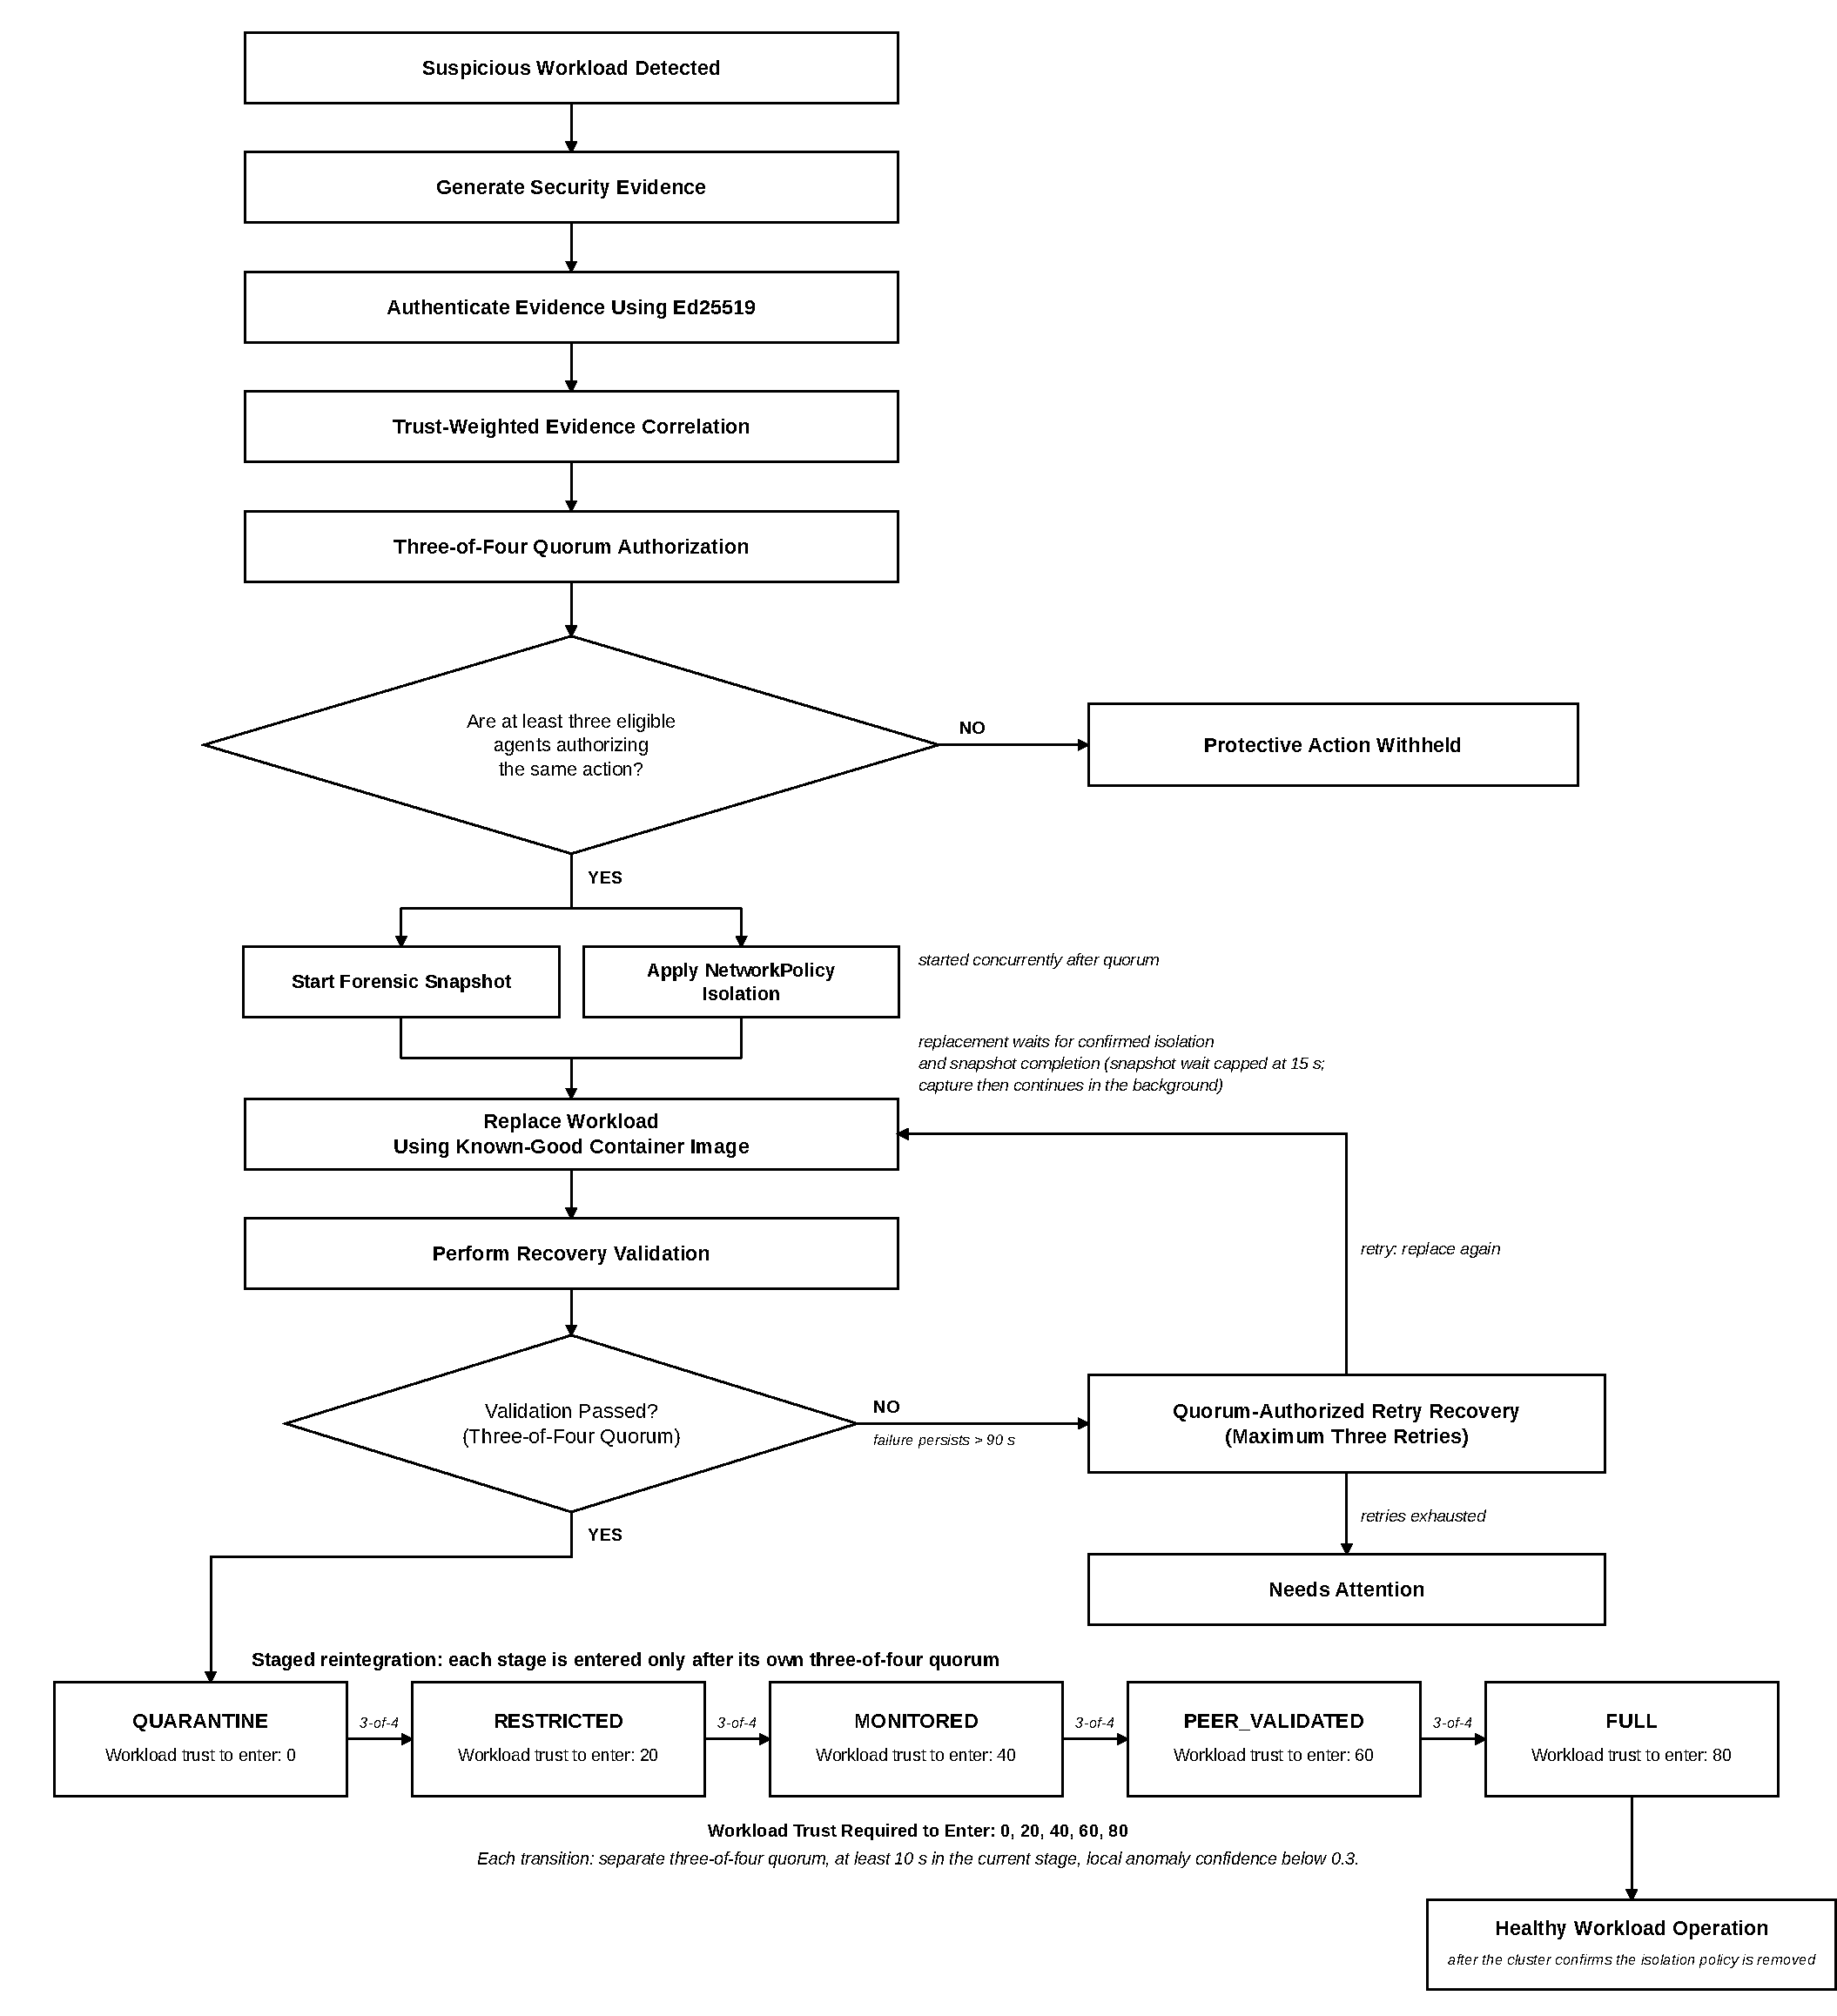
\includegraphics[width=0.95\textwidth]{fig2_workflow.pdf}
\caption{Workflow of evidence validation, quorum-authorized containment, known-good workload replacement, recovery validation, and staged reintegration.}
\label{fig:flow}
\end{figure*}

\subsubsection{Snapshot and isolation}
When the \action{CONTAIN} quorum commits, the executing agent starts a forensic snapshot of the workload and applies a NetworkPolicy called \texttt{resilience-isolate-<workload>}; both actions start at the same time. The replacement waits until the isolation is confirmed in the cluster and the snapshot has completed, but the wait for the snapshot is bounded to 15\,s. Afterwards, the replacement proceeds and the snapshot keeps running in the background; hence there might be an incomplete snapshot when the old pod is deleted.

\subsubsection{Replacement}
The workload is redeployed from the configured known-good image with the Recreate deployment strategy, so that the existing instance is not re-used. The agents are ranked per incident, and a lower-ranked agent waits 3\,s times its rank before acting. Actions are idempotent, and in case of an unclear outcome the agent re-reads the result from the cluster.

\subsubsection{Validation}
Each agent validates the replacement independently: (i) the health endpoint returns HTTP~200; (ii) the instance identifier differs from the one recorded at containment; (iii) if a baseline manifest is loaded, the reported file hashes match it exactly; and (iv) the agent's own anomaly confidence for the workload is below 0.3. An agent casts a \action{VALIDATE} vote only if all four conditions are satisfied, and three eligible agents must do so. These criteria do not establish the identity of the workload: condition (ii) only shows that a different instance is running, and the hashes in (iii) are provided by the workload itself.

\subsubsection{Retries}
If validation fails continuously for 90\,s, or the replacement is still not ready 90\,s after deployment, the agents vote \action{RETRY\_RECOVERY}. Every retry requires its own quorum of three agents, follows a new snapshot of the failed instance, and waits for a back-off that starts at 15\,s and doubles up to 120\,s. There may be at most three retries, so the total number of attempts is at most four. Afterwards, the workload remains quarantined and is flagged as requiring human intervention. Individual failed Kubernetes calls are retried by a separate mechanism, at most ten times with a bounded back-off, before the operation is abandoned.

\subsubsection{Staged reintegration}
Once the validation quorum has completed, the workload enters the \stage{QUARANTINE} stage and moves through \stage{RESTRICTED}, \stage{MONITORED} and \stage{PEER\_VALIDATED} before reaching \stage{FULL}. Every transition requires its own three-agent quorum. An agent votes for the next stage only if the workload has been in its current stage for at least 10\,s, the workload trust has reached the threshold of the next stage (20, 40, 60 and 80 for the four transitions), and its own anomaly confidence is below 0.3. Each stage applies a NetworkPolicy that becomes less restrictive, and \stage{FULL} removes it. A workload at \stage{FULL} counts as healthy only after the cluster confirms that the policy is gone.

Workload trust is each agent's health score for a workload. It decreases by 10 per second while the agent's own observation is 0.5 or more and increases by 2 per second otherwise; it is set to zero whenever a containment commits.

\begin{table}[!t]
\caption{Recovery and Reintegration Parameters (Defaults)}
\label{tab:recov}
\centering\small
\begin{tabularx}{\columnwidth}{@{}Y l@{}}
\toprule
Parameter & Value \\
\midrule
Snapshot wait limit & 15\,s \\
Validation timeout / replacement-ready timeout & 90\,s / 90\,s \\
Recovery retries (maximum attempts) & 3 (4) \\
Retry back-off & 15\,s, doubling, capped at 120\,s \\
Kubernetes-call retries & at most 10, 2--30\,s back-off \\
Reintegration stages & 5 \\
Workload trust needed to enter a stage & 0, 20, 40, 60, 80 \\
Minimum time in a stage & 10\,s \\
Anomaly confidence limit to advance & below 0.3 \\
Workload trust: loss / recovery & 10 / 2 per s \\
\bottomrule
\end{tabularx}
\end{table}

\subsection{Prototype and configuration}
Our prototype is implemented in Python~3.11 and uses gRPC~1.84, Protocol Buffers~7.36, the \texttt{cryptography} library~50.0 for Ed25519 and the certificates, and the Kubernetes Python client~36.0. Each agent maintains a hash-chained local decision log. Calico enforces the NetworkPolicies, and the operator dashboard uses only the Python standard library. The default configurations are specified in Tables~\ref{tab:trustq} and~\ref{tab:recov}. The six workloads serve synthetic records created with Synthea~\cite{synthea}.

\section{Experimental Setup}
Two environments were used for the experiments and one additionally for taking screenshots only; the results are kept separate from each other (Fig.~\ref{fig:testbed}).

\begin{figure*}[!t]
\centering
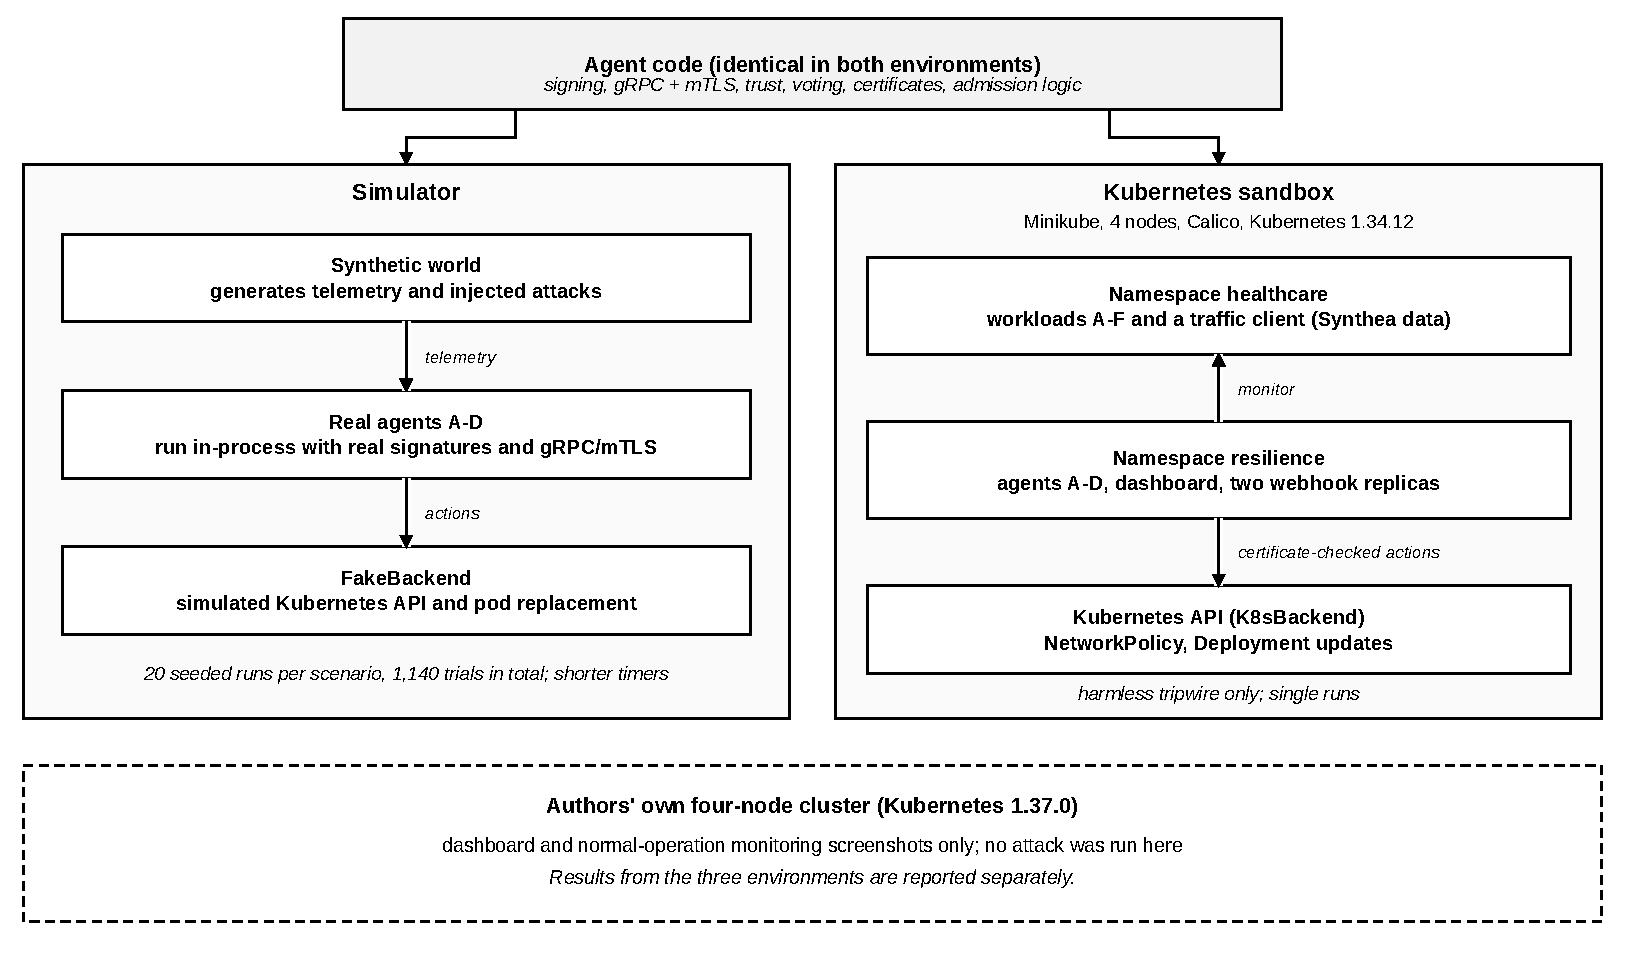
\includegraphics[width=0.8\textwidth]{fig3_testbed.pdf}
\caption{Experimental testbed. The same agent code runs in the simulator and in the Kubernetes sandbox; the authors' own cluster was used only for normal-operation monitoring screenshots.}
\label{fig:testbed}
\end{figure*}

\textbf{Simulator.} The simulator runs the real agent code, including signatures, gRPC with mutual TLS, trust, voting, certificates and the admission logic, within a synthetic world that produces telemetry and a simulated Kubernetes backend. The simulator uses shorter timers than the cluster (for example 3\,s per stage instead of 10\,s), so its times are not wall-clock predictions. Every experiment is run 20 times with constant seeds, except the mixed run (30 genuine and 30 benign trials); in all, 1\,140 seeded trials were executed without errors. Because the simulator is predominantly deterministic, the variance between runs is small and understates what a real cluster would show.

\textbf{Kubernetes sandbox.} A four-node Minikube cluster with Calico (Minikube~1.39, Kubernetes~1.34.12, Calico~3.32) was created in a cloud sandbox. It runs the six workloads, four agents, the dashboard and two webhook replicas. The only attack launched in this environment was a benign operator-triggered tripwire: a single line added to a marker file in a single workload. In addition, the authors' own four-node cluster (Kubernetes~1.37.0) was used to capture screenshots of the monitoring dashboard during normal operation; no attack was run on that cluster.

\textbf{Data.} The workloads use patient records generated by Synthea. The detector consumes telemetry, not records, so the data provide application context only and are not an intrusion detection benchmark.

\begin{table}[!t]
\caption{Software Environment}
\label{tab:software}
\centering\small
\begin{tabularx}{\columnwidth}{@{}p{0.36\columnwidth} Y@{}}
\toprule
Component & Version \\
\midrule
Language & Python 3.11 \\
RPC and serialization & gRPC 1.84.0, Protocol Buffers 7.36.2 \\
Signatures and certificates & \texttt{cryptography} 50.0.1 (Ed25519, ECDSA P-256) \\
Kubernetes client & \texttt{kubernetes} 36.0.3 \\
Sandbox cluster & Kubernetes 1.34.12, Minikube 1.39, Calico 3.32 \\
Authors' own cluster & Kubernetes 1.37.0 (monitoring only) \\
Synthetic data & Synthea \\
\bottomrule
\end{tabularx}
\end{table}

\textbf{Scenarios and metrics.} The simulation scenarios are a multi-signal application compromise, a single-signal attack, a slow-burn attack, a validation-retry scenario (the first replacement fails validation), a lying agent, $k$ compromised or silent agents, agent crashes, a centralized-controller baseline, and a mixture of genuine attacks and benign traffic spikes. We report detection, isolation, recovery and full-access times measured from the start of the attack, the false-alarm rate (an alarm in a benign trial), the false-isolation rate (a benign workload isolated), the missed-isolation rate, and counts with 95\% Wilson intervals.

\section{Results}
\subsection{Overall behavior}
In all four main scenarios (20 runs each), all 80 runs went through detection, isolation, recovery and reintroduction to full access. In the multi-signal application compromise scenario, the median time to isolate is 1.2\,s (simulator time) and the return to normal access takes 18.5\,s, primarily due to the four staged steps. Table~\ref{tab:key} lists the headline numbers, and Table~\ref{tab:timing} and Fig.~\ref{fig:timing} give the distributions of times. The slow-burn attack, which starts weak and builds up, takes longest to isolate (median 9.7\,s, maximum 21.5\,s) since the agents need some time to accumulate evidence. The validation-retry scenario takes longer to reach full access (29.1\,s) due to one failed validation and the back-off period.

\begin{table}[!t]
\caption{Key Results (Simulator Unless Stated)}
\label{tab:key}
\centering\small
\begin{tabularx}{\columnwidth}{@{}Y l@{}}
\toprule
Measure & Result \\
\midrule
Runs reaching full access (4 scenarios) & 80/80 \\
Median time to isolate, app compromise & 1.2\,s \\
Median time to full access, app compromise & 18.5\,s \\
Healthy workload isolated, one lying agent & 0/20 \\
Healthy workload isolated, three lying agents & 20/20 \\
Real attack contained, two agents alive & 0/20 \\
Benign transients: alarm / isolated & 29/30 / 15/30 \\
Sandbox cluster, tripwire to normal access & 83\,s (single run) \\
\bottomrule
\end{tabularx}
\end{table}

\begin{table}[!t]
\caption{Times per Scenario, Simulator Seconds, Median (IQR), 20 Runs Each; All 80 Runs Reached Full Access}
\label{tab:timing}
\centering\scriptsize
\setlength{\tabcolsep}{3pt}
\begin{tabularx}{\columnwidth}{@{}p{1.7cm} Y Y Y Y@{}}
\toprule
Scenario & Detect & Isolate & Recover & Full access \\
\midrule
App compromise & 0.3 (0.2--0.3) & 1.2 (1.0--1.4) & 3.7 (3.4--3.8) & 18.5 (18.3--18.8) \\
Single signal & 0.6 (0.3--0.8) & 1.9 (1.3--2.1) & 4.4 (3.8--4.6) & 19.2 (18.6--19.5) \\
Slow burn & 0.4 (0.2--0.5) & 9.7 (6.4--12.2) & 12.2 (8.9--14.7) & 26.2 (23.3--28.7) \\
Validation retry & 0.1 (0.1--0.3) & 1.2 (1.0--1.3) & 3.6 (3.5--3.7) & 29.1 (28.7--29.3) \\
\bottomrule
\end{tabularx}
\end{table}

\begin{figure*}[!t]
\centering
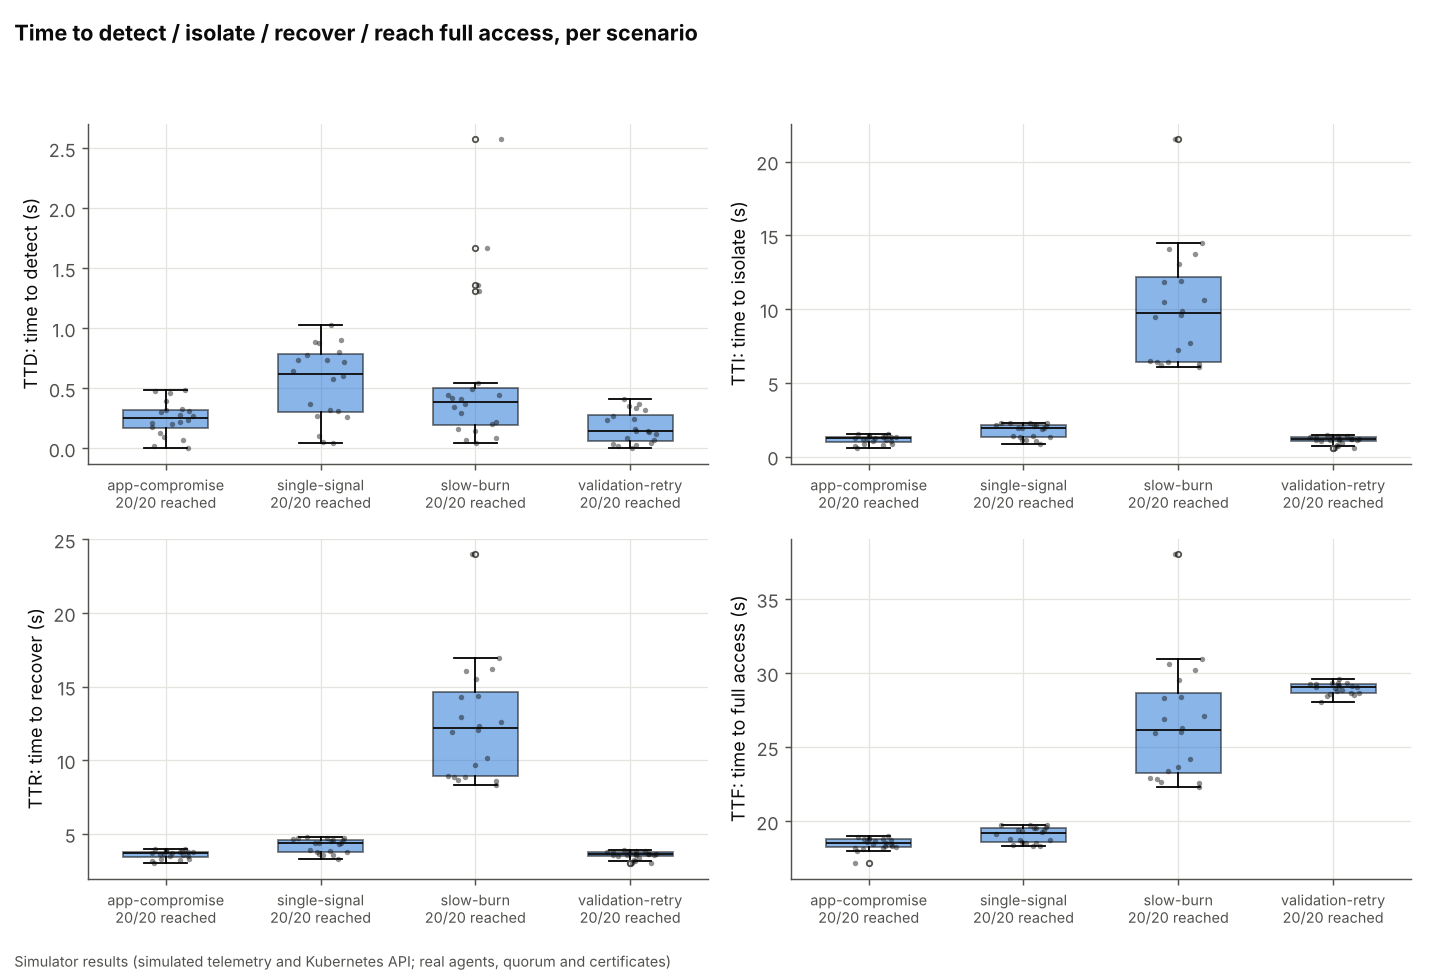
\includegraphics[width=0.62\textwidth]{timing.png}
\caption{Time to detect, isolate, recover and reach full access in the four simulated scenarios (20 runs each; simulator results).}
\label{fig:timing}
\end{figure*}

\subsection{A lying agent}
In this experiment, one agent signs false evidence about a normal workload (the login service). All of the signatures and identities of this agent were validated, and the other three agents did not vote to contain the workload, since each of them found it normal. The workload was never isolated (0/20, 95\% CI 0--16\%). The other three agents marked the lying agent as SUSPECT after a median of 22.5\,s and stopped counting its votes about two seconds later (Fig.~\ref{fig:trust}). The trust in this agent fell to zero in all of the runs. Once the liar was restored, its trust rose at 0.5 per second and was only about 35 after ninety seconds, never again going above 50. Note that in the first 20 seconds or so the protection comes from the quorum, not from trust, which has not yet been reduced.

\begin{figure*}[!t]
\centering
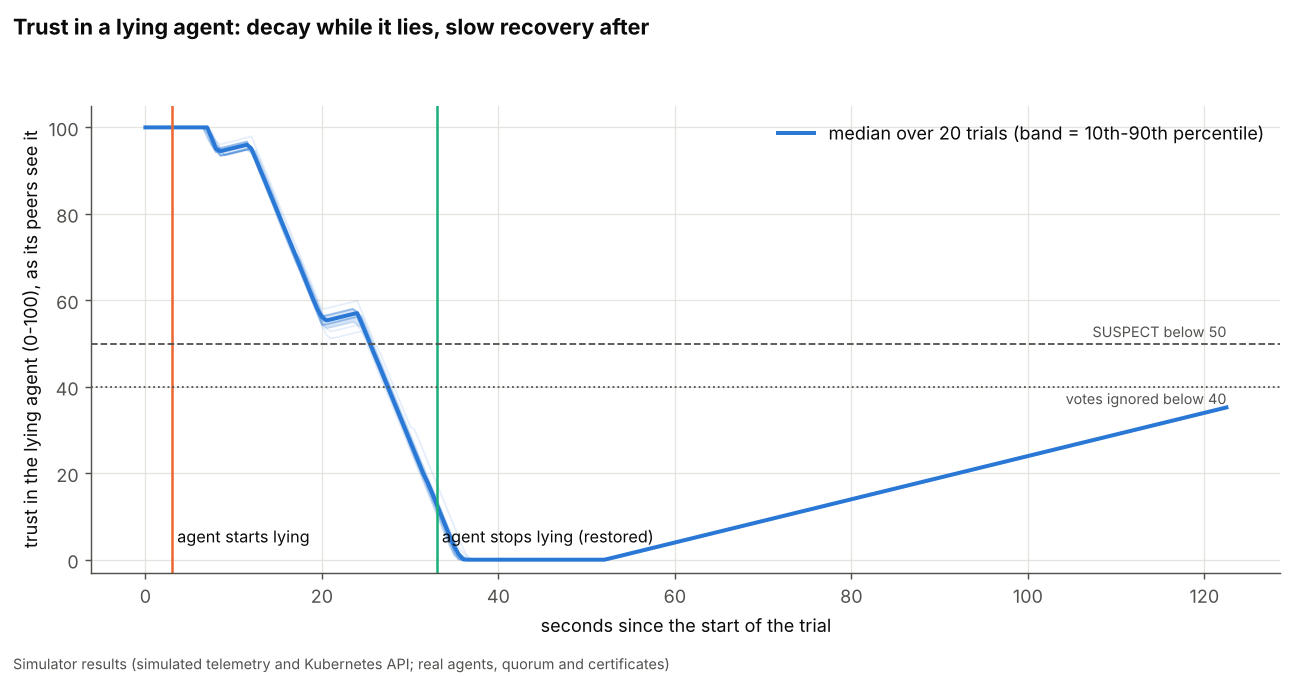
\includegraphics[width=0.62\textwidth]{trust.png}
\caption{Trust that the honest agents place in an agent that lies and later stops lying. The line is the median over 20 runs and the band is the 10th--90th percentile; simulator results.}
\label{fig:trust}
\end{figure*}

\subsection{Quorum boundary, crashes, and a central controller}
Table~\ref{tab:quorum} and Fig.~\ref{fig:faulttol} show the results for experiments in which the number of compromised or silent agents is varied. The scheme holds up against a single compromised agent (two, in case the other two honest agents do not notice anything) and fails where it has to fail. In 20 out of 20 runs, three liars managed to isolate a healthy workload. In addition, in 20 out of 20 runs, two liars plus one honest agent that saw a weak real blip managed to isolate a healthy workload. With two silent agents, there was nothing to contain (0/20). With three out of four agents active, the whole cycle was executed (20/20). In the case of a central controller, a lying controller isolated a healthy workload every time (20/20) and left 79\% of the workloads available over the testing period, while a controller crash resulted in an uncontained real attack (0/20). The distributed scheme showed neither problem in these experiments. The comparison is shown in Fig.~\ref{fig:dvc}. It is relevant to our baseline controller only and cannot be generalized to centralized detection systems in general.

\begin{figure*}[!t]
\centering
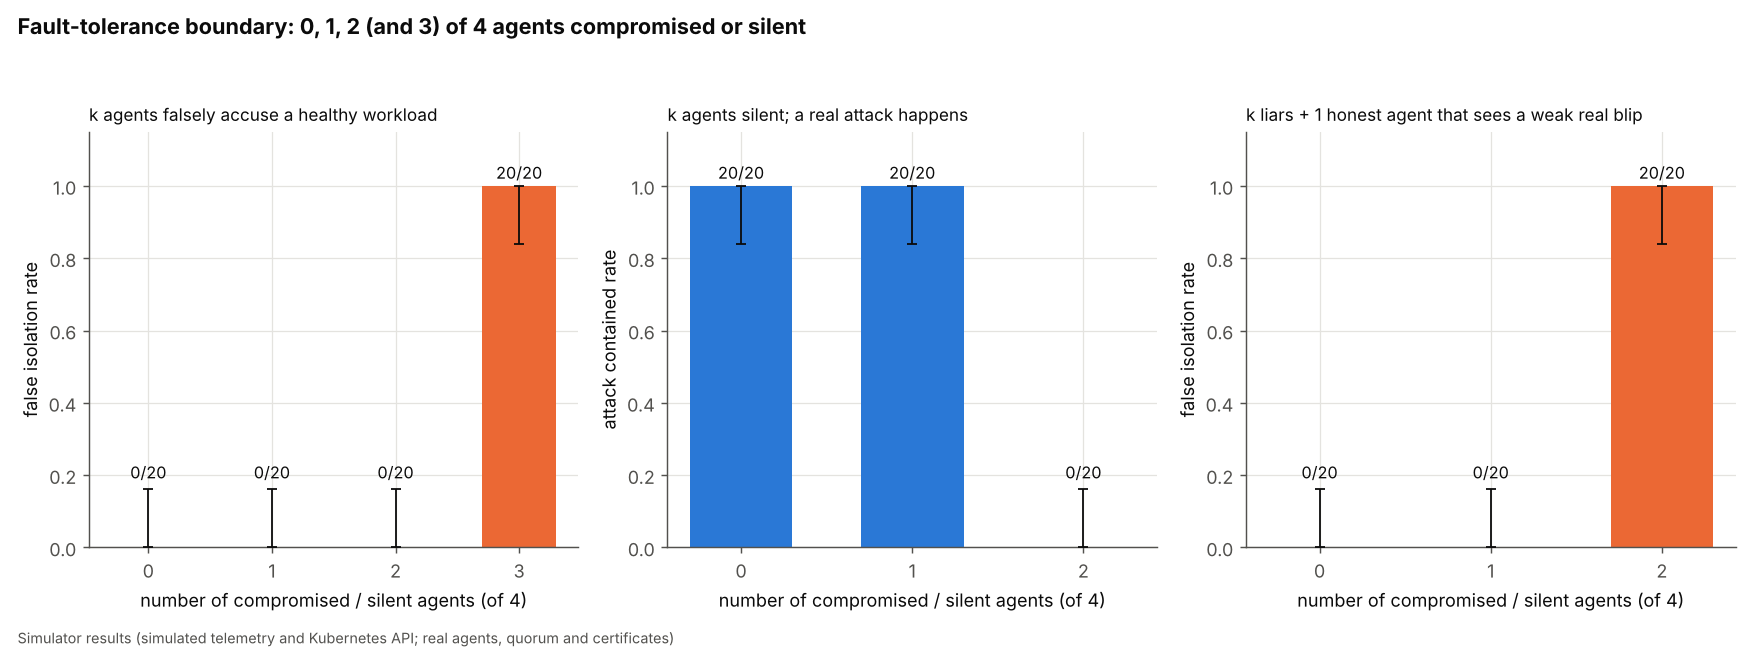
\includegraphics[width=0.85\textwidth]{faulttol.png}
\caption{Fault-tolerance boundary: false isolation, containment of a real attack, and false isolation with one honest agent seeing a weak real blip, as the number of compromised or silent agents grows from 0 to 3 (20 runs per bar, 95\% intervals; simulator).}
\label{fig:faulttol}
\end{figure*}

\begin{figure*}[!t]
\centering
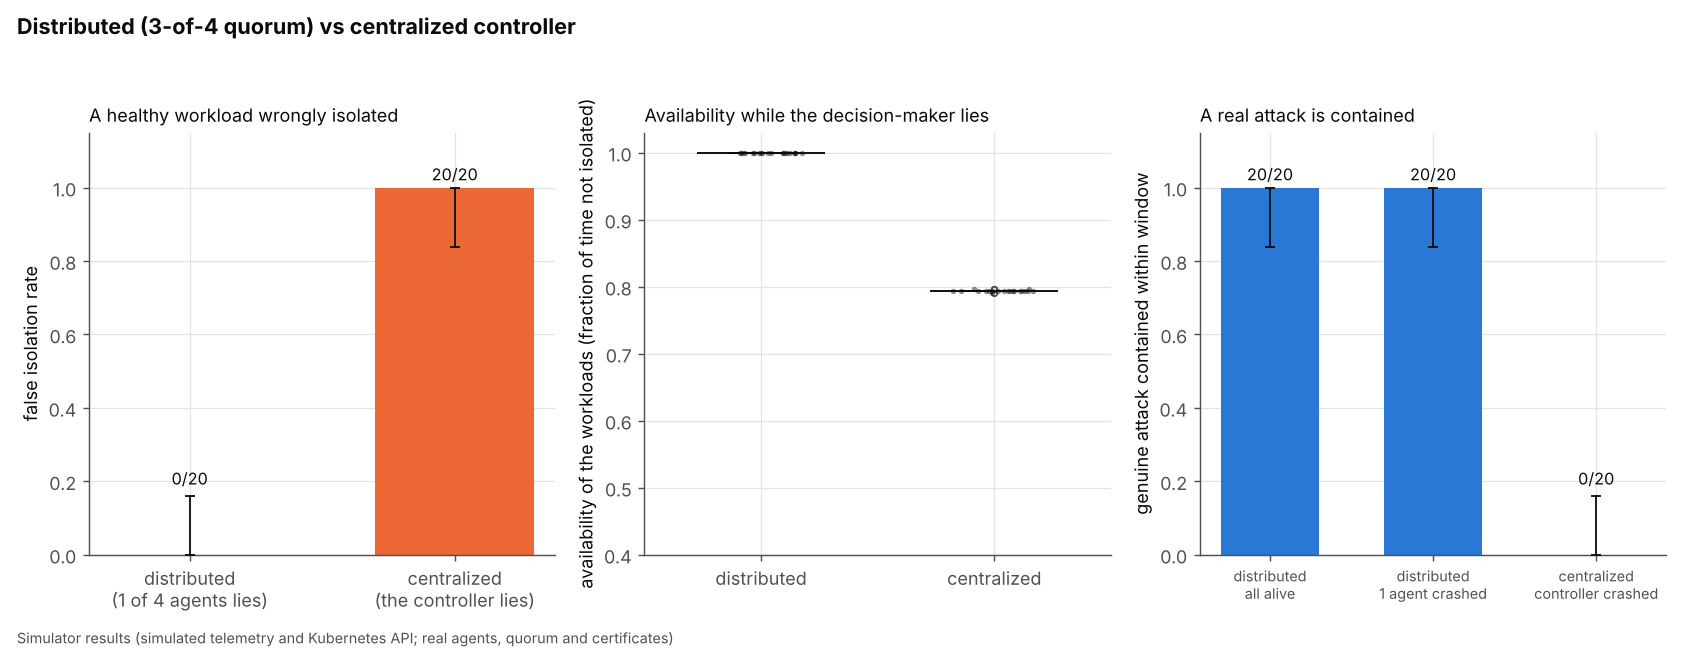
\includegraphics[width=0.85\textwidth]{dvc.png}
\caption{Distributed three-of-four design against our centralized-controller baseline: a healthy workload wrongly isolated, availability while the decision-maker lies, and containment of a real attack (20 runs each; simulator).}
\label{fig:dvc}
\end{figure*}

\begin{table}[!t]
\caption{Quorum Behaviour Under Compromised, Silent and Crashed Agents (20 Runs per Row, Simulator)}
\label{tab:quorum}
\centering\footnotesize
\begin{tabularx}{\columnwidth}{@{}Y l@{}}
\toprule
Condition & Outcome \\
\midrule
$k$=0, 1, 2 liars accuse a healthy workload & False isolation 0/20 each \\
$k$=3 liars accuse a healthy workload & False isolation 20/20 \\
$k$=0, 1 liars + 1 honest agent sees a weak blip & False isolation 0/20 each \\
$k$=2 liars + 1 honest agent sees a weak blip & False isolation 20/20 \\
$k$=0, 1 agents silent, real attack & Contained 20/20 each \\
$k$=2 agents silent, real attack & Contained 0/20 \\
4 / 3 / 2 agents alive, real attack & Contained 20/20 / 20/20 / 0/20 \\
One agent withholds all its votes & Contained 20/20, median 1.5\,s \\
Central controller lies (distributed: one agent lies) & False isolation 20/20 (0/20) \\
Central controller crashed (distributed: one agent crashed) & Contained 0/20 (20/20) \\
\bottomrule
\end{tabularx}
\end{table}

\subsection{False alarms and false isolations}
The mixed run used 30 genuine attacks (random combinations of the three attack signals) and 30 benign transients (either brief spikes in outbound connections seen by one to four agents, or long weak bursts). All 30 genuine attacks triggered an alarm and led to isolation, so there were no misses (0 out of 30). Of the 30 benign cases, 29 triggered an alarm (97\%) and 15 resulted in an isolation (50\%, 95\% CI 33--67\%). The precision at the isolation level was 67\%, the recall was 100\%, and therefore $F_1$ is 0.80. Table~\ref{tab:mixed} and Fig.~\ref{fig:mixed} provide the details, and the breakdown is revealing: none of the 12 benign transients that were seen by just one or two agents was ever isolated, but 15 of the 18 seen by three or four agents were isolated. A threshold detector cannot differentiate between a spike that all agents see and an attack, so the quorum only helps where the benign interference is partial. In a real cluster, all four agents monitor the same endpoints, and hence spikes will usually be seen by all four. Therefore, the 50\% should be viewed as a stress test with our chosen benign mixture rather than an expected rate in production.

\begin{table}[!t]
\caption{Mixed Run: Detection and Isolation Outcomes (Simulator)}
\label{tab:mixed}
\centering\small
\begin{tabularx}{\columnwidth}{@{}Y l@{}}
\toprule
Metric & Result \\
\midrule
Genuine attacks: raised an alarm & 30/30 \\
Genuine attacks: isolated (missed isolation) & 30/30 (0/30) \\
Benign transients: raised an alarm & 29/30 (97\%) \\
Benign transients: isolated (false isolation) & 15/30 (50\%) \\
\quad seen by 1--2 agents & 0/12 isolated \\
\quad seen by 3--4 agents & 15/18 isolated \\
Precision / recall at isolation & 67\% / 100\% \\
$F_1$ at isolation & 0.80 \\
\bottomrule
\end{tabularx}
\end{table}

\begin{figure}[!t]
\centering
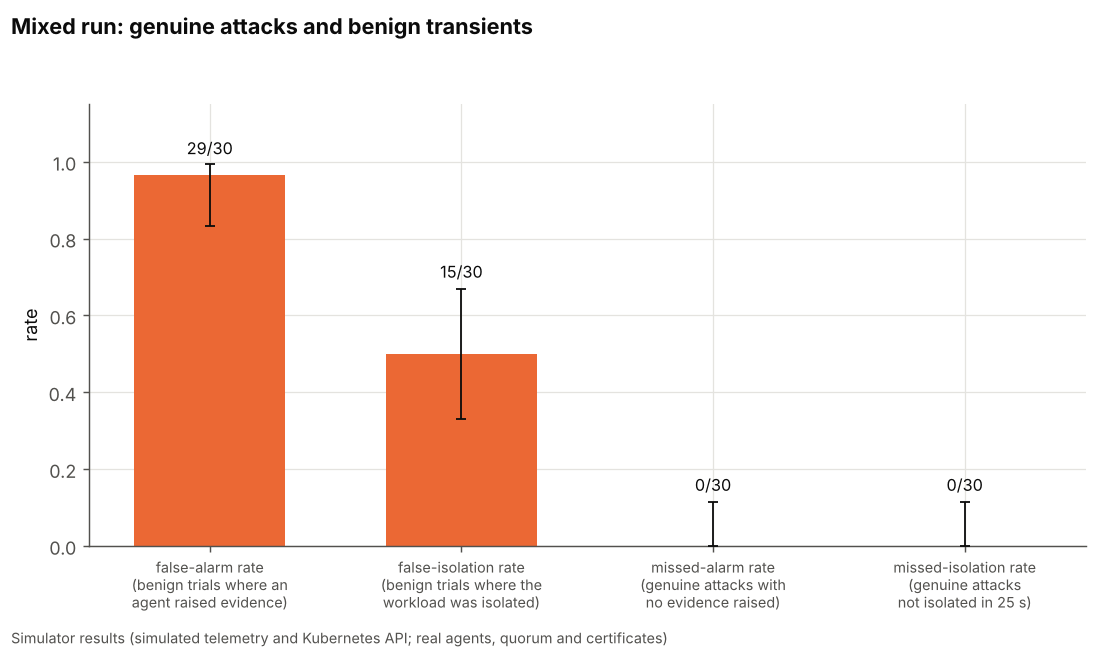
\includegraphics[width=\columnwidth]{mixed.png}
\caption{Mixed run of 30 genuine attacks and 30 benign transients (simulator). Bars show rates with 95\% confidence intervals.}
\label{fig:mixed}
\end{figure}

\subsection{What the staged return gives us}
We compared the real design with two evaluation-only baseline designs using the same seeds (Fig.~\ref{fig:baselines}). When a dormant implant became active during the staged return, none of the runs had the workload at full access while compromised (0/14), compared with ten out of fourteen runs with an immediate return; in both cases the workload was contained again. The cost is time: a median of 18.3\,s to full access for the staged return compared with 8.5\,s for the immediate one. If the implant only wakes up after the staged return would have finished, the gates do not help (5/6 versus 6/6). A baseline in which a single agent decides isolated a healthy workload in twenty out of twenty runs after just one false accusation or a short spike, compared with zero out of twenty with the three-of-four design.

\begin{figure*}[!t]
\centering
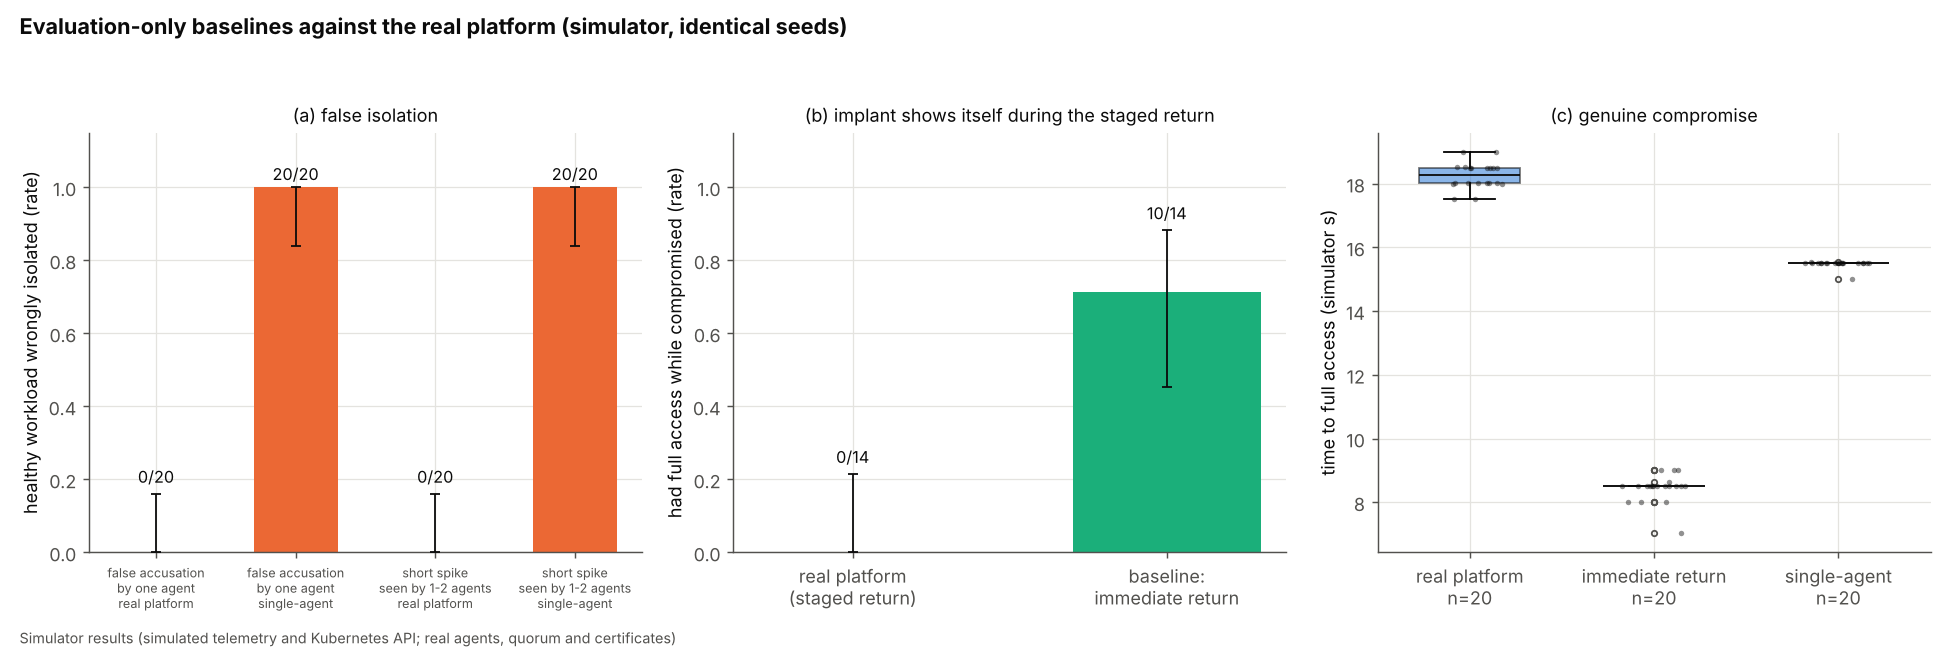
\includegraphics[width=0.85\textwidth]{baselines.png}
\caption{Staged return and quorum against two evaluation-only baselines, identical seeds (simulator). (a) healthy workloads wrongly isolated, (b) implant active during the return, (c) time to full access.}
\label{fig:baselines}
\end{figure*}

\subsection{Overhead}
In the simulation, each idle agent consumed roughly 0.1\% of one core and 2.3\,MB of extra memory. This increased to about 1.0\% and 4.2\,MB per agent during an attack and recovery. These numbers are indicative only.

\subsection{Kubernetes sandbox}
The sandbox cluster exercised the parts that the simulator cannot: the real API server, Calico enforcement and the webhook. Table~\ref{tab:sandbox} shows the checks performed. A tripwire written to workload E (laboratory results) produced a \action{CONTAIN} quorum signed by agents A--D two seconds later, an isolation, a new pod, a \action{VALIDATE} quorum, and four stage transitions, each with a quorum certificate that passed the webhook. The workload had normal access again after 83\,s; most of that time was the 30\,s pod termination grace period and the four 10\,s dwells. Workload F took about 82\,s, and repeating the test on E after a deployment upgrade went through the same process. These are single runs of a benign trigger in one sandbox, so they show that the pipeline works end to end under real conditions, not how it performs. The sandbox runs also exposed four flaws: three in our verification scripts, and one genuine issue, where the webhook kept its old configuration after the upgrade and rejected the isolation of the new workloads. All were fixed and covered by tests.

\begin{table}[!t]
\caption{Sandbox-Cluster Checks (Kubernetes 1.34.12, Minikube, Calico)}
\label{tab:sandbox}
\centering\footnotesize
\begin{tabularx}{\columnwidth}{@{}Y l@{}}
\toprule
Check & Result \\
\midrule
RBAC probe per workload (6 workloads) & 27/27 pass each \\
Admission webhook (3 workloads) & 7/7 pass each \\
Webhook down, agent request still refused & 8/8 pass \\
Calico isolation (2 workloads) & 16/16 pass each \\
Baseline file manifest, all workloads & 6/6 match \\
Tripwire on E, quorum to normal access & 83\,s (A--D signed) \\
Tripwire on F, quorum to normal access & about 82\,s \\
\bottomrule
\end{tabularx}
\end{table}

\subsection{Live monitoring}
On the authors' own cluster, the dashboard reported four of four agents connected and six of six workloads healthy, with telemetry about one second old (Fig.~\ref{fig:live}). Each agent displayed its trust in the other agents and its evidence scores, and five checked files per workload, all consistent with the baseline. These screenshots show normal operation. No attack was launched on this cluster; therefore, all the attack-response numbers come from the simulator or the sandbox.

\begin{figure*}[!t]
\centering
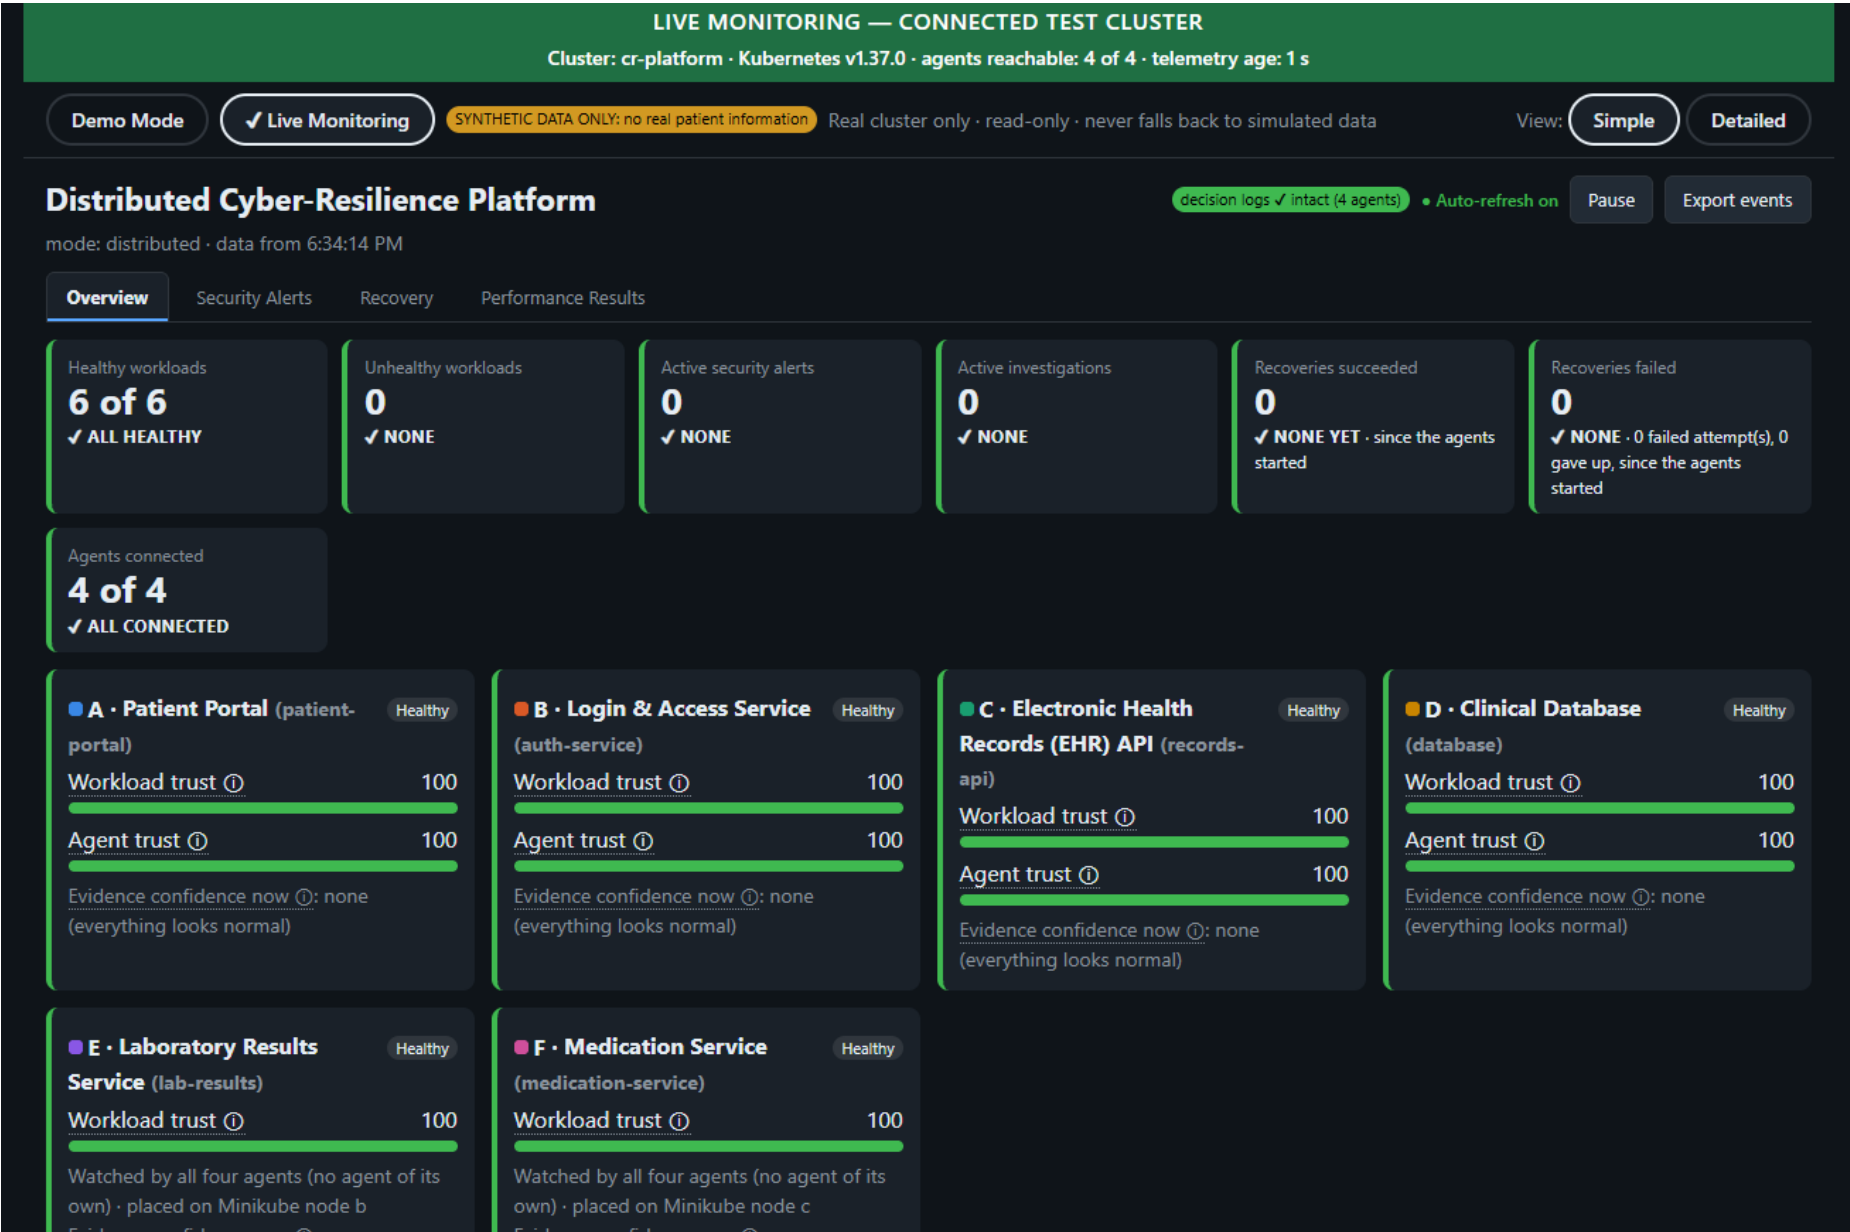
\includegraphics[width=0.75\textwidth]{live.png}
\caption{Dashboard connected to the authors' four-node Minikube cluster (Kubernetes 1.37.0): four of four agents reachable, six of six workloads healthy, synthetic data only. This is normal operation, not an attack.}
\label{fig:live}
\end{figure*}

\section{Discussion and Limitations}
\label{sec:limits}
The results support a narrow claim. Requiring three of four agents blocks a single liar and a single false alarm, an agent crash does not stop the response, and a replaced workload that is brought back in stages gives an implant less room than an immediate return. However, they do not show that the system detects attacks efficiently. The detector consists of static rules, 97\% of benign spikes triggered an alarm, and whether an alarm became an isolation depended on whether three agents saw the same disturbance.

We regard the following limitations as significant.
\begin{enumerate}
\item \textbf{Mainly simulated.} Almost all of the attack-response statistics come from the simulator with synthetic telemetry and a fake Kubernetes backend, with faster timers and almost no timing noise. The sandbox shows that the real pipeline executes, in one case of a harmless trigger.
\item \textbf{Poor detection.} Static thresholds, no learning, no real healthcare attack traces, and a high number of false alarms in our benign setup.
\item \textbf{Self-reported telemetry.} Process lists, file hashes, instance identifiers and health are self-reported by the workload through unauthenticated HTTP. A compromised workload can report inaccurate information, and there is no way to authenticate the workload's identity. File-hash validation only takes place when a baseline manifest is loaded.
\item \textbf{Not Byzantine consensus.} Three or more cooperating agents can approve a false action and obtain a valid certificate, as can be seen from Table~\ref{tab:quorum}.
\item \textbf{Keys and certificates.} The PKI is static, and there is no key rotation or revocation. The certificate verifier supports a ``consumed'' check, but neither the agents nor the webhook use it, so certificate replay protection relies on the epoch and expiry time.
\item \textbf{Clocks.} Messages whose timestamp differs by more than 15\,s are rejected and the delivering peer loses trust, so an honest agent with an incorrect clock is penalized.
\item \textbf{Evidence preservation.} The wait for the snapshot is capped at 15\,s, so a snapshot may be incomplete when the replacement starts.
\item \textbf{Scope of the webhook and audit.} The webhook only applies to one service account in one namespace, not to other administrators. The decision log is hash-chained but stored only locally on each agent and not anchored elsewhere.
\item \textbf{Scale and data.} The experiments used four agents, six workloads and twenty runs per test case, with Synthea data; no real patient data were used, and this is not a clinical or production evaluation.
\item \textbf{Hand-chosen parameters.} Trust rates, vote thresholds and timers were set by hand, without sensitivity analysis or optimization.
\end{enumerate}
Future work should start with the detector (thresholds, representative benign and attack traces), then telemetry authentication and attestation, key rotation, and a consensus protocol (if tolerance of more than one bad agent is required).

\section{Conclusion}
We described and implemented a prototype in which four peer agents validate evidence, monitor each other's credibility and authorize containment, validation, retries and each reintegration step only after three of them have agreed. In simulation it completed every attack-response run, prevented one malicious agent from isolating a healthy workload, continued to operate despite one agent failure, and outperformed centralized and single-agent control policies on our test cases. A Minikube/Calico sandbox completed the entire contain--replace--validate--reintegrate sequence with quorum certificates verified by an admission webhook. The same experiments defined the boundaries: three compromised agents overrule the quorum, two live agents cannot act, the staged reintegration is about twice as slow as an immediate one (18.3\,s against 8.5\,s), and the rule-based detector raises many false alarms, about half of which resulted in isolation in our benign setting. The system's shortcomings are the detector and the unauthenticated telemetry, and these are the areas that require further development.

\section*{Acknowledgment}
The authors would like to acknowledge the help of Dr.\ Swetha P.\,C.\ during the course of the project, and the Head of the Department and the Principal of BMS College of Engineering for providing the necessary facilities. We would also like to acknowledge the Synthea project for the synthetic data generator.

\section*{Declarations}
\textbf{Funding:} None. \textbf{Conflict of interest:} None declared. \textbf{Ethics:} No human subjects or real patient data were used; all health data are synthetic. \textbf{Data and code availability:} From the corresponding author upon request. \textbf{Author contributions:} To be filled in by the authors prior to submission.

\section*{Declaration of Generative AI and AI-Assisted Technologies in the Writing Process}
During the preparation of this work the authors used Claude (Anthropic) to analyze the project source code, to draft and edit parts of the text, to generate the LaTeX source, and to draw the architecture, workflow and testbed diagrams. After using this tool, the authors reviewed and edited the content as needed and take full responsibility for the content of the publication.

\begin{thebibliography}{99}
\bibitem{zhou10} C. V. Zhou, C. Leckie, and S. Karunasekera, ``A survey of coordinated attacks and collaborative intrusion detection,'' \emph{Comput. Secur.}, vol. 29, no. 1, pp. 124--140, Feb. 2010.
\bibitem{vasilo15} E. Vasilomanolakis, S. Karuppayah, M. M{\"u}hlh{\"a}user, and M. Fischer, ``Taxonomy and survey of collaborative intrusion detection,'' \emph{ACM Comput. Surv.}, vol. 47, no. 4, 2015.
\bibitem{li22} W. Li, W. Meng, and L. F. Kwok, ``Surveying trust-based collaborative intrusion detection: State-of-the-art, challenges and future directions,'' \emph{IEEE Commun. Surveys Tuts.}, vol. 24, no. 1, pp. 280--305, 2022.
\bibitem{elshoush11} H. T. Elshoush and I. M. Osman, ``Alert correlation in collaborative intelligent intrusion detection systems---A survey,'' \emph{Appl. Soft Comput.}, vol. 11, no. 7, pp. 4349--4365, Oct. 2011.
\bibitem{balas98} J. Balasubramaniyan, J. O. Garcia-Fernandez, D. Isacoff, E. Spafford, and D. Zamboni, ``An architecture for intrusion detection using autonomous agents,'' in \emph{Proc. 14th Annu. Comput. Security Appl. Conf. (ACSAC)}, 1998, pp. 13--24.
\bibitem{josang07} A. J{\o}sang, R. Ismail, and C. Boyd, ``A survey of trust and reputation systems for online service provision,'' \emph{Decis. Support Syst.}, vol. 43, no. 2, pp. 618--644, Mar. 2007.
\bibitem{kamvar03} S. D. Kamvar, M. T. Schlosser, and H. Garcia-Molina, ``The EigenTrust algorithm for reputation management in P2P networks,'' in \emph{Proc. 12th Int. Conf. World Wide Web (WWW)}, 2003, pp. 640--651.
\bibitem{lamport82} L. Lamport, R. Shostak, and M. Pease, ``The Byzantine generals problem,'' \emph{ACM Trans. Program. Lang. Syst.}, vol. 4, no. 3, pp. 382--401, Jul. 1982.
\bibitem{flp85} M. J. Fischer, N. A. Lynch, and M. S. Paterson, ``Impossibility of distributed consensus with one faulty process,'' \emph{J. ACM}, vol. 32, no. 2, pp. 374--382, Apr. 1985.
\bibitem{castro99} M. Castro and B. Liskov, ``Practical Byzantine fault tolerance,'' in \emph{Proc. 3rd Symp. Operating Syst. Design Implement. (OSDI)}, 1999, pp. 173--186.
\bibitem{castro02} M. Castro and B. Liskov, ``Practical Byzantine fault tolerance and proactive recovery,'' \emph{ACM Trans. Comput. Syst.}, vol. 20, no. 4, pp. 398--461, Nov. 2002.
\bibitem{jarkas25} O. Jarkas, R. Ko, N. Dong, and R. Mahmud, ``A container security survey: Exploits, attacks, and defenses,'' \emph{ACM Comput. Surv.}, vol. 57, no. 7, 2025.
\bibitem{patel13} A. Patel, M. Taghavi, K. Bakhtiyari, and J. Celestino J{\'u}nior, ``An intrusion detection and prevention system in cloud computing: A systematic review,'' \emph{J. Netw. Comput. Appl.}, vol. 36, no. 1, pp. 25--41, Jan. 2013.
\bibitem{modi13} C. Modi, D. Patel, B. Borisaniya, H. Patel, A. Patel, and M. Rajarajan, ``A survey of intrusion detection techniques in cloud,'' \emph{J. Netw. Comput. Appl.}, vol. 36, no. 1, pp. 42--57, Jan. 2013.
\bibitem{nist190} M. P. Souppaya, J. Morello, and K. Scarfone, ``Application container security guide,'' NIST, Gaithersburg, MD, USA, Special Publication 800-190, Sep. 2017.
\bibitem{garcia09} P. Garc{\'\i}a-Teodoro, J. D{\'\i}az-Verdejo, G. Maci{\'a}-Fern{\'a}ndez, and E. V{\'a}zquez, ``Anomaly-based network intrusion detection: Techniques, systems and challenges,'' \emph{Comput. Secur.}, vol. 28, no. 1--2, pp. 18--28, 2009.
\bibitem{bhuyan14} M. H. Bhuyan, D. K. Bhattacharyya, and J. K. Kalita, ``Network anomaly detection: Methods, systems and tools,'' \emph{IEEE Commun. Surveys Tuts.}, vol. 16, no. 1, pp. 303--336, 2014.
\bibitem{khraisat19} A. Khraisat, I. Gondal, P. Vamplew, and J. Kamruzzaman, ``Survey of intrusion detection systems: Techniques, datasets and challenges,'' \emph{Cybersecurity}, vol. 2, Art. no. 20, 2019.
\bibitem{rfc8032} S. Josefsson and I. Liusvaara, ``Edwards-curve digital signature algorithm (EdDSA),'' RFC 8032, Jan. 2017.
\bibitem{rfc8446} E. Rescorla, ``The transport layer security (TLS) protocol version 1.3,'' RFC 8446, Aug. 2018.
\bibitem{rfc5280} D. Cooper \emph{et al.}, ``Internet X.509 public key infrastructure certificate and certificate revocation list (CRL) profile,'' RFC 5280, May 2008.
\bibitem{nist61} A. Nelson, S. Rekhi, M. Souppaya, and K. Scarfone, ``Incident response recommendations and considerations for cybersecurity risk management: A CSF 2.0 community profile,'' NIST, Special Publication 800-61 Rev.~3, Apr. 2025.
\bibitem{nist207} S. Rose, O. Borchert, S. Mitchell, and S. Connelly, ``Zero trust architecture,'' NIST, Special Publication 800-207, Aug. 2020.
\bibitem{csf2} NIST, ``The NIST cybersecurity framework (CSF) 2.0,'' NIST Cybersecurity White Paper 29, Feb. 2024.
\bibitem{synthea} J. Walonoski \emph{et al.}, ``Synthea: An approach, method, and software mechanism for generating synthetic patients and the synthetic electronic health care record,'' \emph{J. Amer. Med. Inform. Assoc.}, vol. 25, no. 3, pp. 230--238, 2018.
\end{thebibliography}

\end{document}
